% Author: Max Melching, 2025
% Lots of styling inspiration from: https://tikz.net/relativity_minkowski_diagram/
\documentclass[border=3pt,tikz]{standalone}

\usepackage{newtxmath}  % Use Times in math mode
\usepackage{tgpagella}  % Use Pagella in text
\usepackage{tikz}
\usepackage{fp}
\usepackage{calc}
\usepackage{pgfkeys}
\usepackage{ifthen}
\usepackage{xcolor}
\usepackage[outline]{contour} % glow around text


\usetikzlibrary{math,arrows.meta,calc,intersections,through,backgrounds,decorations.markings,decorations.pathmorphing}


% -- Styling
\colorlet{lightyellow}{black!10!yellow}  % Mix with 10% of yellow
\colorlet{mydarkred}{red!55!black}
\colorlet{myred}{red!85!black}
\colorlet{mydarkorange}{orange!40!yellow!85!black}
\colorlet{mydarkblue}{blue!50!black}


\tikzset{
    >={Stealth[inset=0,angle'=27]},
    light/.style={
        ->,
        lightyellow,
        line width=0.6,
        decorate,
        decoration={
            snake,
            amplitude=0.5,
            segment length=4.2,
            post length=4.2,
        }
    },
    worldline/.style={
        ->,
        thick,
        black,
    },
    labelledpoint/.style={
        % mydarkred,
        myred,
    },
    simultline/.style={
        mydarkblue,
        dashed,
        % line width=0.4,
        thin,
    }
}


% -- Not styling, this is to Lorentz-transform objects
\tikzset{
    vlorentz/.style={
      cm={1/((1-((#1)*(#1)))^.5,#1*1/((1-((#1)*(#1)))^.5,#1*1/((1-((#1)*(#1)))^.5,1/((1-((#1)*(#1)))^.5,(0,0)}
    },
}



\begin{document}

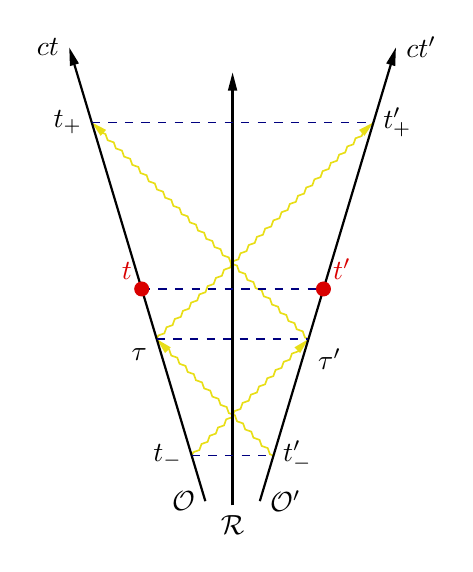
\begin{tikzpicture}[scale=1.1]
	\def\vone{-0.3}
    \def\vtwo{0.3}
    \def\tsignal{1.5}
    \def\initsep{0}

    \def\tmin{1}
    \def\tmax{6}
    
    
    % -- From here on automatic (except you wish to change styling) -----------
    \FPeval{\dopplerone}{((1+\vone)/(1-\vone))^.5}
    \FPeval{\dopplertwo}{((1+\vtwo)/(1-\vtwo))^.5}
    \FPeval{\doppleronetwo}{\dopplertwo/\dopplerone}

    
    \FPeval{\vrelative}{(\vtwo-\vone)/(1-\vone*\vtwo)}
    
    \FPifzero{\vrelative}
        % -- Only initsep is present, just set sensible values
        \FPeval{\vrelativehalf}{0}
        \FPeval{\vreferee}{\vone}
    \else
        \FPeval{\vrelativehalf}{(1-(1-\vrelative*\vrelative)^.5)/\vrelative}
        \FPeval{\vreferee}{(\vone+\vrelativehalf)/(1+\vone*\vrelativehalf)}
    \fi
    

    \begin{scope}[vlorentz=\vone]
        \coordinate (A) at (0, \tsignal);
        \coordinate (E) at (0, \doppleronetwo*\tsignal + \initsep);
        \coordinate (B) at (0, \doppleronetwo*\doppleronetwo*\tsignal + 2*\initsep);
        \coordinate (ABhalf) at ($ (A)!0.5!(B) $);
    \end{scope}

    \begin{scope}[vlorentz=\vtwo]
        \coordinate (C) at (\initsep, \tsignal);
        \coordinate (F) at (\initsep, \doppleronetwo*\tsignal + \initsep);
        \coordinate (D) at (\initsep, \doppleronetwo*\doppleronetwo*\tsignal + 2*\initsep);
        \coordinate (CDhalf) at ($ (C)!0.5!(D) $);
    \end{scope}
    
	
    \draw[light] (A) -- (F);
    \draw[light] (F) -- (B);

	\draw[light] (C) -- (E);
    \draw[light] (E) -- (D);

    
    % -- Observer worldlines
	\draw[worldline, vlorentz=\vone] (0, \tmin) node[left] {$\mathcal{O}$} -- (0, \tmax) node[left] {$ct$};
	\draw[worldline, vlorentz=\vtwo] (\initsep, \tmin) node[right] {$\mathcal{O}'$} -- (\initsep, \tmax) node[right] {$ct'$};
	\draw[worldline, vlorentz=\vreferee] ({\initsep/2}, \tmin) node[below] {$\mathcal{R}$} -- ({\initsep/2}, \tmax);

    % -- Lines of Simultaneity
    \draw[simultline] (A) -- (C);
    \draw[simultline] (B) -- (D);
    \draw[simultline] (E) -- (F);
    \draw[simultline] (ABhalf) -- (CDhalf);

    % -- Point halfway between emission and reception
	\draw[fill, labelledpoint] (ABhalf) circle(0.08);
	\draw[fill, labelledpoint] (CDhalf) circle(0.08);

    % -- Labels. Comment if you do not like
    \node[left] at (A) {$t_-$};
    \node[right] at (C) {$t'_-$};

    \node[left] at (B) {$t_+$};
    \node[right] at (D) {$t'_+$};

    \node[above left, labelledpoint] at (ABhalf) {$t$};
    \node[above right, labelledpoint] at (CDhalf) {$t'$};

    \node[below left] at (E) {$\tau$};
    \node[below right] at (F) {$\tau'$};
\end{tikzpicture}



\end{document}